\documentclass{article} % For LaTeX2e
\usepackage{nips14submit_e,times}
\usepackage{amsmath}
\usepackage{amsthm}
\usepackage{amssymb}
\usepackage{mathtools}
\usepackage{hyperref}
\usepackage{url}
\usepackage{algorithm}
\usepackage[noend]{algpseudocode}
%\documentstyle[nips14submit_09,times,art10]{article} % For LaTeX 2.09

\usepackage{graphicx}
\usepackage{caption}
\usepackage{subcaption}

\def\eQb#1\eQe{\begin{eqnarray*}#1\end{eqnarray*}}
\def\eQnb#1\eQne{\begin{eqnarray}#1\end{eqnarray}}
\providecommand{\e}[1]{\ensuremath{\times 10^{#1}}}
\providecommand{\pb}[0]{\pagebreak}
\DeclarePairedDelimiter\ceil{\lceil}{\rceil}
\DeclarePairedDelimiter\floor{\lfloor}{\rfloor}

\newcommand{\E}{\mathrm{E}}
\newcommand{\Var}{\mathrm{Var}}
\newcommand{\Cov}{\mathrm{Cov}}

\def\Qb#1\Qe{\begin{question}#1\end{question}}
\def\Sb#1\Se{\begin{solution}#1\end{solution}}

\newenvironment{claim}[1]{\par\noindent\underline{Claim:}\space#1}{}
\newtheoremstyle{quest}{\topsep}{\topsep}{}{}{\bfseries}{}{ }{\thmname{#1}\thmnote{ #3}.}
\theoremstyle{quest}
\newtheorem*{definition}{Definition}
\newtheorem*{theorem}{Theorem}
\newtheorem*{lemma}{Lemma}
\newtheorem*{question}{Question}
\newtheorem*{preposition}{Preposition}
\newtheorem*{exercise}{Exercise}
\newtheorem*{challengeproblem}{Challenge Problem}
\newtheorem*{solution}{Solution}
\newtheorem*{remark}{Remark}
\usepackage{verbatimbox}
\usepackage{listings}
\usepackage{mathrsfs}
\title{Functional Analysis: \\
Problem Set II}


\author{
Youngduck Choi \\
CIMS \\
New York University\\
\texttt{yc1104@nyu.edu} \\
}


% The \author macro works with any number of authors. There are two commands
% used to separate the names and addresses of multiple authors: \And and \AND.
%
% Using \And between authors leaves it to \LaTeX{} to determine where to break
% the lines. Using \AND forces a linebreak at that point. So, if \LaTeX{}
% puts 3 of 4 authors names on the first line, and the last on the second
% line, try using \AND instead of \And before the third author name.

\newcommand{\fix}{\marginpar{FIX}}
\newcommand{\new}{\marginpar{NEW}}

\nipsfinalcopy % Uncomment for camera-ready version

\begin{document}


\maketitle

\begin{abstract}
This work contains solutions to the exercises of the problem set II.
\end{abstract}

\bigskip

\begin{question}[1]
\hfill
\begin{figure}[h!]
  \centering
    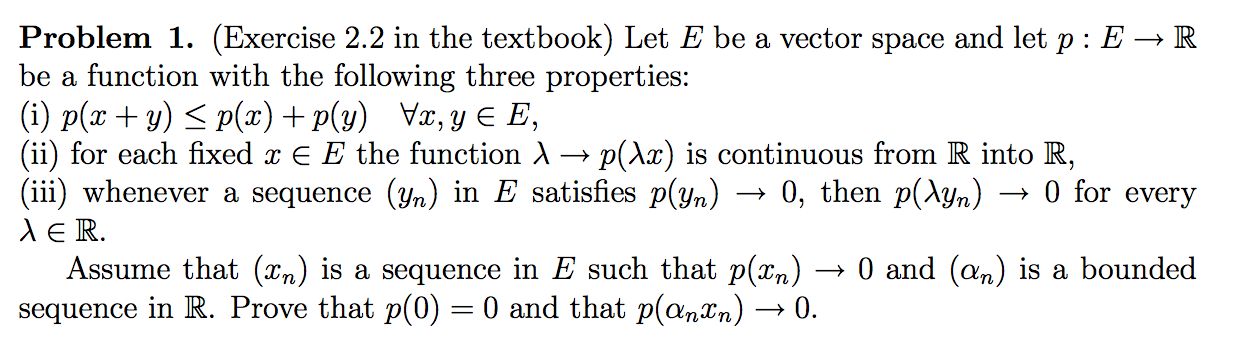
\includegraphics[width=0.7\textwidth]{funcA-h-e2-p1.png}
\end{figure}
\end{question}
\begin{solution} \hfill \\
Fix $\epsilon > 0$. Suppose for sake contradiction that there exists
a subsequence $\{a_{n_k} x_{n_k}\}$ such that 
\eQb
|p(a_{n_k}x_{n_k})| \geq 2\epsilon \>\>\> (*)
\eQe
for all $k \geq 1$
Since $\{a_n\}$ is bounded, 
passing to a further subsequence, and relabeling, we may suppose that
\eQb
|p(a_{n} x_{n}) | \geq 2\epsilon &\text{and}& \lim_{n \to \infty} a_n = a
\eQe
for any $n \geq 1$ and for some $a \in \mathbb{R}$. 
Now, observe that $\phi_k:\mathbb{R} \to \mathbb{R}$ defined by 
\eQb
\lambda &\mapsto& |p(\lambda x_k)| \>\>\> (\lambda \in \mathbb{R})
\eQe
for each $k \geq 1$ is continuous by (ii). Therefore,  
\eQb
F_n &=& \bigcap_{k=n}^{\infty} {\phi_k}^{-1}([-\epsilon,\epsilon])
\eQe
is closed for each $n \geq 1$ ($F_n$ given in the hint). 
By assumption and (iii), it follows that
\eQb
\bigcup_{n} F_n &=& \mathbb{R}
\eQe 
and by Baire-Category, we can choose $n_0 \in \mathbb{N}$ such that there
exists $\lambda_0 \in \mathbb{R}$ and $\delta > 0$ such that 
\eQb
B(\lambda_0,\delta) \subset F_{n_0}.
\eQe
Now, by (i), we obtain
\eQb
p(a_k x_k) &\leq& p((\lambda_0 + a_k - a) x_k) + p((a - \lambda_0) x_k) 
\eQe
and
\eQb
-p(a_k x_k) &\leq& -p((\lambda_0 + a_k - a) x_k) + p((\lambda_0 - a)x_k)
\eQe
for each $k \geq 1$. Now for all $k$ large enough, since $(a - \lambda_0), 
(\lambda_0 - a)$
are fixed constants, we have
\eQb
(\lambda_0 + a_k - a) \in B(\lambda_0,\delta) \>\>\> \text{and} \>\>\> 
|p((a- \lambda_0)|,|p(\lambda_0 - a)| < \epsilon
\eQe
so
\eQb
|p(a_k x_k)| &<& 2\epsilon,
\eQe
which contradicts $(*)$. By (i), $p(0) \leq 2p(0)$, and $p(0) \leq p(x_n) + 
p(-x_n) $ for all $n \geq 1$, so $p(0) \leq 0$. Therefore, $p(0) = 0$. 
\hfill $\qed$ 


\end{solution}

\newpage

\begin{question}[2]
\hfill
\begin{figure}[h!]
  \centering
    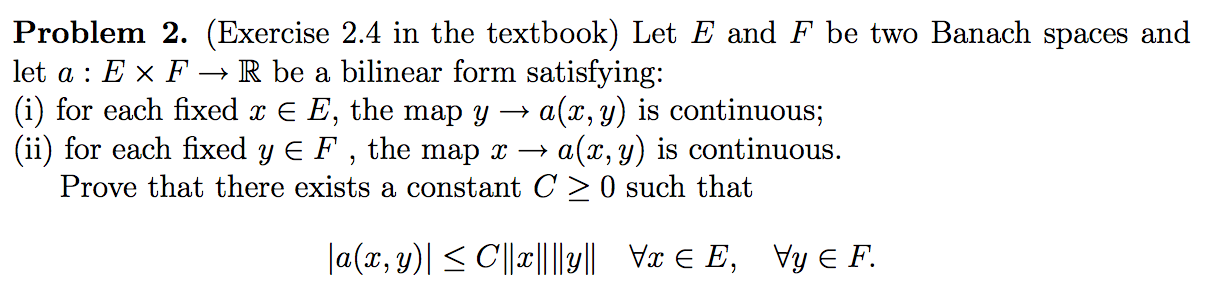
\includegraphics[width=0.7\textwidth]{funcA-h-e2-p2.png}
\end{figure}
\end{question}
\begin{solution} \hfill \\
Define a map $T$ on $E$ by 
\eQb
x \mapsto T_x \>\>\> \text{with} \>\>\> <T_x,y> = a(x,y).
\eQe
By (i), $T_x$ is bounded for all $x \in E$, so $T$ maps $E$
into $F^*$. We now show that $T$ is bounded. 
Fix $y \in F$. Observe that
\eQb
\{ <Tx,y> \> : \> x \in B_{E}(0,1) \} &=& \{ a(x,y) \> : \> x \in B_E(0,1) \}
\eQe
is bounded by (ii). Therefore, by Corollary 2.5, which follows from
Uniform boundedness principle, $T$ is bounded. 
Now, by the boundedness of $T$, there 
exists $C > 0$ such that
\eQb
\sup_{y \in F; ||y|| \neq 0} \dfrac{|a(x,y)|}{||y||} = ||T_x|| \leq C||x||
\eQe
for any $x \in E$, and hence
\eQb
a(x,y) \leq C ||x|| ||y||
\eQe
for any $x \in E$ and $y \in F$. \hfill $\qed$
\end{solution}

\newpage

\begin{question}[3]
\hfill
\begin{figure}[h!]
  \centering
    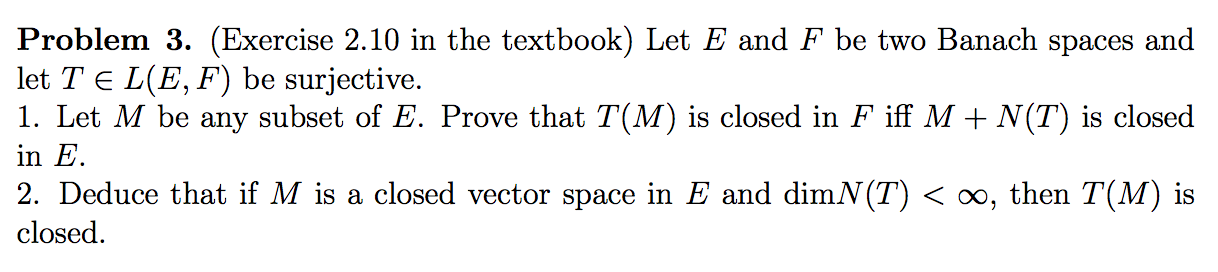
\includegraphics[width=0.7\textwidth]{funcA-h-e2-p3.png}
\end{figure}
\end{question}
\begin{solution} \hfill \\
Suppose that $T(M)$ is closed. Then, by continuity of $T$,
\eQb
M + N(T) = T^{-1}(T(M)) \>\>\> \text{is closed}.
\eQe
Conversely, suppose that $M + N(T)$ is closed. We contend that
\eQb
T((M + N(T))^c) = T(M)^c. \>\>\> (*) 
\eQe 
Let $x \in T(M + N(T)^c)$. Then, there exists $y \in (M + N(T))^c$, 
such that $T(y) = x$. Suppose for sake of contradiction that $x \in T(M)$. 
Then, there exists $x_0 \in M$, such that $T(x_0) = y$, and by linearity of $T$,
$x - x_0 \in N(T)$, so $x \in M + N(T)$, a contradiction. 
For the other inclusion, let $x \in T(M)^c$. By surjectivity of $T$,
there exists $z \in E$ such that $T(z) = x$. Suppose for sake of contradiction
that $z = m + n$ with some $m \in M$ and $n \in N(T)$. By linearity of $T$,
\eQb
x = T(z) = T(m), 
\eQe 
which contradicts that $x \in T(M)^c$. Therefore, (*) is true.
To conclude, observe that,
by open mapping theorem, $T(M)^c$ is open, so $T(M)$ is closed.
Now, (ii) follows from the problem 5 and (i). \hfill $\qed$

\end{solution}

\newpage

\begin{question}[4]
\hfill
\begin{figure}[h!]
  \centering
    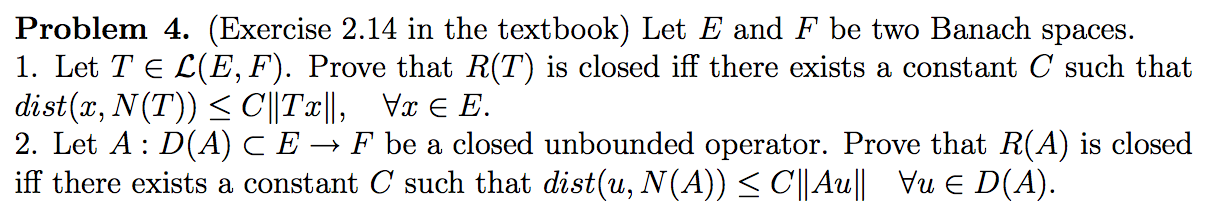
\includegraphics[width=0.7\textwidth]{funcA-h-e2-p4.png}
\end{figure}
\end{question}
\begin{solution} \hfill \\
\textbf{(1)}
Let $\tilde{E} = E / N(T)$, $\pi$ be the canonical quotient map,
and $\tilde{T}:E / N(T) \to F$ such that $T = \tilde{T} \circ \pi$.
From definition, we know that $\tilde{T}$ is linear, injective, and $R(T) 
= R(\tilde{T})$. 

\smallskip

Suppose the given estimate holds. We claim that $R(\tilde{T})$ is closed, then by 
$R(T) = R(\tilde{T})$, we will be done. Observe that 
\eQb
||[x]|| = d(x,N(T)) \leq C||Tx|| = C||\tilde{T}[x]|| (*)
\eQe  
for all $x \in E$. Suppose $\{y_n\} \subset R(\tilde{T})$ such that $y_n \to y$ for some
$y$. Then, there exists 
$\{[x_n]\} \subset \tilde{E}$. By the above estimate, $\{[x_n]\}$ is
cauchy, and by continuity $\tilde{T}[x_n] \to \tilde{T}[x]$ where $[x]$ is the
limit of $\{[x_n]\}$. Therefore, $R(\tilde{T})$ is closed. 

Suppose $R(T)$ is closed. Then, $R(\tilde{T})$ is closed, and hence Banach.
Since $\tilde{T}$ is bijective, by Corollary 2.7, $\tilde{T}^{-1}$ is continuous so 
we again have (*).

\bigskip

\textbf{(2)} Consider $D(A)$ with graph norm. Then, as $A$ is closed, $D(A)$ is 
Banach. Since graph norm only increases the norm from each norm, $T$ is bounded
and by (1) we are done.



\end{solution}

\newpage

\begin{question}[5]
\hfill
\begin{figure}[h!]
  \centering
    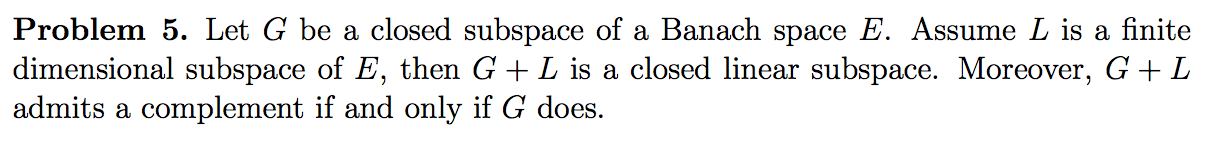
\includegraphics[width=0.7\textwidth]{funcA-h-e2-p5.png}
\end{figure}
\end{question}
\begin{solution} \hfill \\
Let $\pi$ be the canonical projection of $E$ onto $E / G$. As $L$
is finite dimensional space, we see that $\pi(L)$ is finite dimensional, hence
closed.  
By continuity of $\pi$, it follows that $\pi^{-1}(\pi(L)) = G + L$ is closed.

\bigskip

Suppose $G+L$ admits a complement $A$ in $E$. Since $G \cap L$ is finite dimensional,
it admits a complement $B$ in $L$. $A+B$ is closed by (i). 
We claim that $A +B$ is the complement of $G$. If $g \in A+B \cap G$, then
$g = a+b$ for some $b \in B$ and $a \in A$. By re-arranging, we see that 
$a = 0$ and $g = 0$. Therefore, it follows that for any $x \in A$, we can express it
as an unique sum of an element in $A+B$ and $G$, so $A+B$ is a complement of $G$.



\bigskip

Suppose $G$ admits a complement $H$ in $E$. Let $\pi_G$ and $\pi_H$ be canonical  
projections of $G$ and $H$ respectively. Observe that
$\pi_H(L)$ is finite dimensional, so it admits a complement $A \subset H$
in $H$. We claim that $A$ is a complement of $G + L$. Note that $A$ is closed
trivially. Suppose $x \in A \cap G+L$. Then, $x = g+l$ for some $g \in G$ 
and $l \in L$. By projection properties, one can see that $x = 0$, and again 
see that $x$ can be written as a unique sum of an element in $G+L$ and $A$
which completes the proof. \hfill $\qed$


\end{solution}

\newpage

\begin{question}[6]
\hfill
\begin{figure}[h!]
  \centering
    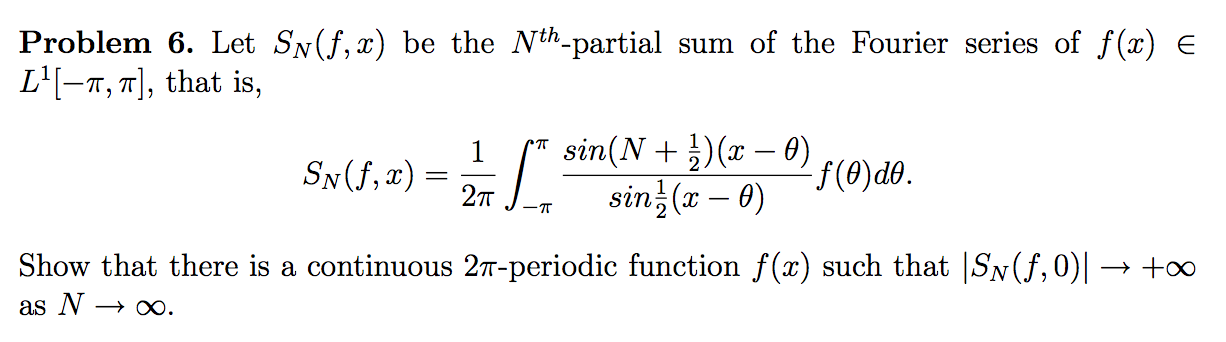
\includegraphics[width=0.7\textwidth]{funcA-h-e2-p6.png}
\end{figure}
\end{question}
\begin{solution} \hfill \\
For convenience, we identify $\mathbb{T}$ with $[0,2\pi]$ and consider $0$ as the point,
where we study the divergence.
Let $\{\phi_n\}$ be a collection of continuous, linear functionals (standard property
of Fourier series), defined on $C(\mathbb{T})$ given by 
\eQb
\phi_n(f) &=& S_n(f,0)
\eQe
for all $f \in C(\mathbb{T})$ and $n \in \mathbb{N}$. Suppose for a moment that
$\{\phi_n\}$ are not uniformly bounded. Then, by uniform boundedness principle,
there exists $f \in C(\mathbb{T})$ such that $\{\phi_n(f)\}$ is not bounded. 

We now show that $\{|\phi_n|\}$
is not bounded. Since $|\sin(t)| \leq t$
for any $t \in [0,2\pi]$, 
\eQb
\int_{0}^{2\pi} |\dfrac{\sin(n+\frac{1}{2})x}{\sin(\frac{x}{2})}| dx &\geq&
\int_{0}^{2\pi} |\sin(n + \frac{1}{2})x| \frac{2}{x} dx = \int_{0}^{2\pi(n+\frac{1}{2})}
|\sin(x)| \dfrac{2}{x} dx \\
&\geq& \sum_{k=1}^{n} \dfrac{1}{k} \int_{2\pi(k-1)}^{2\pi k} |\sin(x)|dx \geq 
\sum_{k=1}^{n} \dfrac{1}{k}  
\eQe
for all $n \in \mathbb{N}$. 
The above estimate shows that the $L^1$ norms of the n-th Dirichlet kernels associated 
with $\phi_n$ diverges to $\infty$. Now, it is well-known 
that the functional norm of $\phi_n$
is exactly the $L^1$ norm of the n-th Dirichlet kernel for all $n \in \mathbb{N}$.
This can be formally shown by considering the sign of the kernel as the continuous
function, and using DCT to swap the order of limit and integration.
\hfill $\qed$

\end{solution}

\newpage

\begin{question}[7]
\hfill
\begin{figure}[h!]
  \centering
    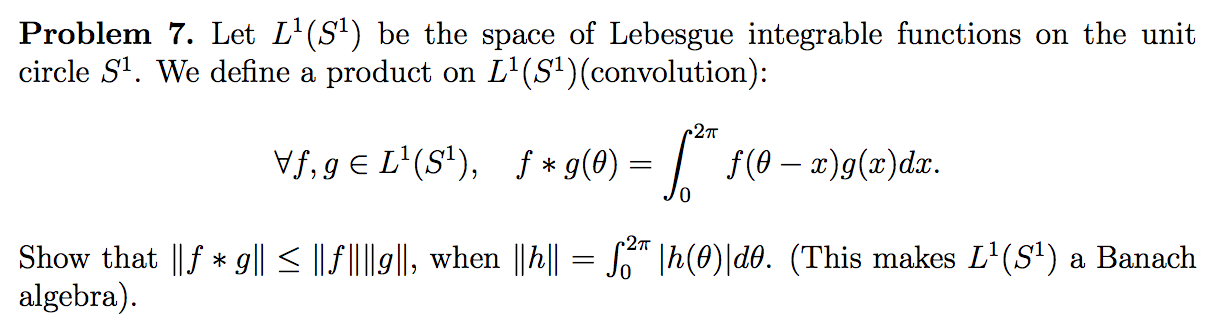
\includegraphics[width=0.7\textwidth]{funcA-h-e2-p7.png}
\end{figure}
\end{question}
\begin{solution} \hfill \\
By Tonelli's theorem and the translation invariance property of Lebesgue measure,
\eQb
||f * g|| &=& \int_{0}^{2\pi} |\int_{0}^{2\pi} f(t - x)g(x) dx | dt  
\leq  \int_{0}^{2\pi}\int_{0}^{2\pi} |f(t-x)g(x)| dx dt \\
&=& \int_{0}^{2\pi} \int_{0}^{2\pi} |f(t-x)g(x)| dt dx 
= \int_{0}^{2\pi} |g(x)| \int_{0}^{2\pi} |f(t-x)| dt dx \\
&=& ||f|| \int_{0}^{2\pi} |g(x)| = ||f|| ||g|| 
\eQe
for any $f,g \in L^1(S^1)$. \hfill $\qed$ 


\end{solution}

\newpage

\begin{question}[8]
\hfill
\begin{figure}[h!]
  \centering
    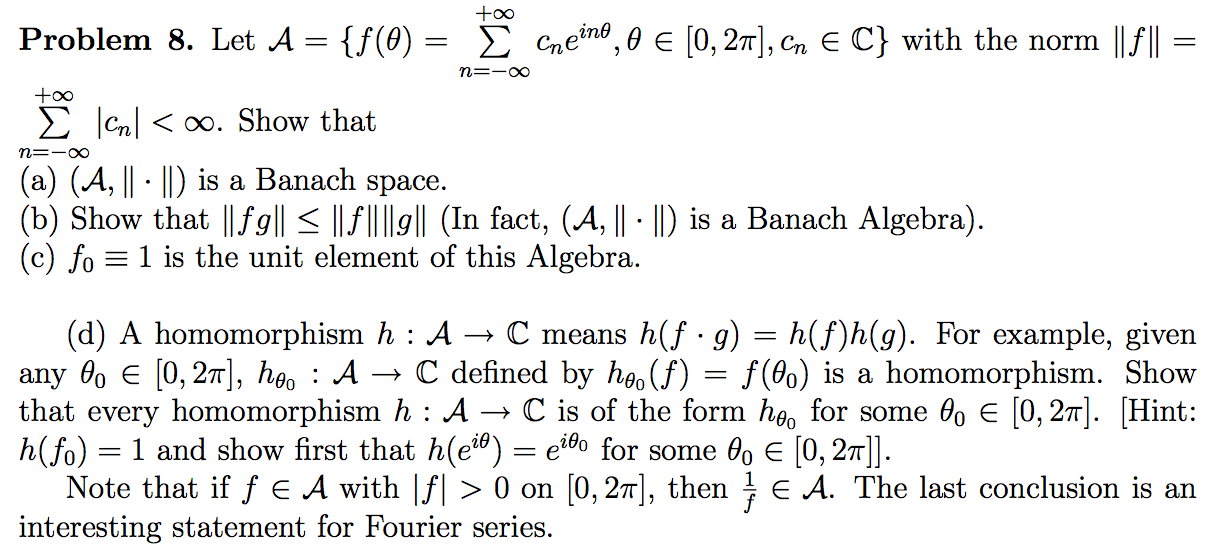
\includegraphics[width=0.7\textwidth]{funcA-h-e2-p8.png}
\end{figure}
\end{question}
\begin{solution} \hfill \\
\end{solution}





\end{document}
